\documentclass[a4paper,10pt, english]{article}

\usepackage{amssymb}
\usepackage{amsmath}
\usepackage{enumitem}
\usepackage{graphicx}





\newcommand{\D}{\displaystyle}

\newtheorem{theo}{Theorem}[section]
\newcommand{\R}{\mathbb{R}}



\newtheorem{prop}[theo]{Proposition}


\begin{document}



\section{Some facts about the system}

Consider the dynamical system 

\begin{equation}
\label{s1}
\D
\dot{x_i} = x_i \phi(x_i)\left(\prod_{j=1}^{N} \left(\frac{x_j}{x_i}\right)^{v_{ij}} - \prod_{j=1}^{N}\left(\frac{x_j}{x_i}\right)^{w_{ij}} \right), \qquad i=1,\ldots, N,
\end{equation}
$$
x_i(0) = x_{i0}, \quad \mbox{\---} \quad \mbox{initial conditions, }
$$
where $x$ \--- the state, $\phi(x) = \sqrt{x(x_{max}-x)}$. 

In the case when $\mathbf{v} = \{v_{ij}\}_{i,j=1, \ldots, N}$ and $\mathbf{w} = \{w_{ij}\}_{i,j=1, \ldots, N}$ are stochastic matrices, meaning $\sum_{j=1}^{N}v_{ij} = \sum_{j=1}^{N}w_{ij} = 1$ the system (\ref{s1}) becomes
\begin{equation}
\label{s2}
\D
\dot{x_i}  = \phi(x_i)\left(\prod_{j=1}^{N} \left(x_j\right)^{v_{ij}} - \prod_{j=1}^{N}\left(x_j\right)^{w_{ij}} \right), \qquad i=1,\ldots, N.
\end{equation}
The above dynamical system (\ref{s2}) has an equilibrium when
\begin{equation}
\label{s3}
\D
 \phi(x_i)\left(\prod_{j=1}^{N} \left(x_j\right)^{v_{ij}} - \prod_{j=1}^{N}\left(x_j\right)^{w_{ij}} \right) = 0, \qquad i=1,\ldots, N.
\end{equation}

Taking the logarithm of (\ref{s3}) and denoting $y_i = \lg{x_i}$, $\Delta_{ij} = v_{ij} - w_{ij}$ the system (\ref{s3}) transforms to the following

\begin{equation}
\label{s4}
\D
\sum_{j=1}^{N}\Delta_{ij}y_j = 0, \qquad i=1,\ldots, N.
\end{equation}

Therefore, (\ref{s3}) holds if  (\ref{s4}) holds. Clearly, (\ref{s4}) holds for $y=(y_1, y_2, \ldots, y_N) = (0, 0, \ldots, 0)$, i.e. the sytem (\ref{s2}) has an equilibrium in 
$x=(x_1, x_2, \ldots, x_N) = (1, 1, \ldots, 1)$. Other equilibrium points are only possible when the matrix $\mathbf{\Delta} = \{\Delta_{ij}\}_{i,j=1, \ldots, N}$ is singular.
Which is true when matrices $\mathbf{v}$ and $\mathbf{w}$ are stochastic, since adding up all the columns in $\mathbf{\Delta}$ will result in a zero column.
Note that for a singular matrix $\mathbf{\Delta}$ there are infinitely many equilibriums, because there are infinitely many solutions of the system (\ref{s4}). 
Let's find those equilibriums. Apart of  $x = (0, 0, \ldots, 0)$ and $x = (1, 1, \ldots, 1)$ (\ref{s3}) holds for $x_1 =  x_2 = \ldots = x_N$ because then (\ref{s3}) become
$$
\D
 \phi(x)\left(x^1 - x^1\right) = 0, \qquad i=1,\ldots, N.
$$
where $x = x_i$, $\forall i=1,\ldots, N$.

Therefore, the equilibriums of the system (\ref{s2}) constitute a susbpace $U_e\subset\mathbb{R}^N$, $U_e = \{x = (x_1, x_2, \ldots, x_N)\in\mathbb{R}^N | x_1 =  x_2 = \ldots = x_N = x^e\in\mathbb{R}\}$.


\newpage
Let's look at the nature of those equilibriums. The linearization of the system around a poin $x\in U_e$ has the form
$$
\dot{\delta x} = \Delta f(x) \delta x,
$$
where $\D \Delta f(x) = \frac{\partial f_i(x)}{\partial x_j}$, $i, j =1, 2, \ldots, N.$

$$
\frac{\partial f_i(x)}{\partial x_j} = v_{ij}x^{v_{ij}-1}\prod_{k=1, k\neq j}^{N}x^{v_{ik}} - w_{ij}x^{w_{ij}-1}\prod_{k=1, k\neq j}^{N}x^{w_{ik}} =
$$
$$
v_{ij}x^{\sum_{k=1}^{N}v_{ik} - 1} - w_{ij}x^{\sum_{k=1}^{N}w_{ik} - 1} = v_{ij} - w_{ij} = \Delta_{ij},
$$
therefore,  $\Delta f(x) = \mathbf{\Delta}$ for all $x\in U_e$.

Note that the matrix $\mathbf{\Delta}$ always has a zero eignvalue, because the $|\mathbf{\Delta}| = 0$. This implies that the equilibriums $x\in U_e$ are not asymptotically stable.

\newpage
\section{Numerical observations}
\subsection{Example 1}


Consider the case $N=3$, the time horizon $T = 100$, $x_{max} = 1$,
$$
\mathbf{v} = 
\left(
\begin{matrix}
0 & 0.5 & 0.5 \\
0.5 & 0 & 0.5 \\
0.5 & 0.5 & 0 \\
\end{matrix}
\right),
$$

$$
\mathbf{w} = 
\left(
\begin{matrix}
0.5 & 0.5 & 0 \\
0 & 0.5 & 0.5 \\
0.5 & 0 & 0.5 \\
\end{matrix}
\right).
$$
Here $\mathbf{v}$ and $\mathbf{w}$ are stochastic, then $|\mathbf{\Delta}| = 0$. Therefore the problem has more than one equilibrium. 
Let us have a look at the graph of the solution with the initial conditions $x_0 = (0.3\quad 0.6\quad 0.9)$.

\begin{figure}[ht]
\label{fig_c1}
\centering
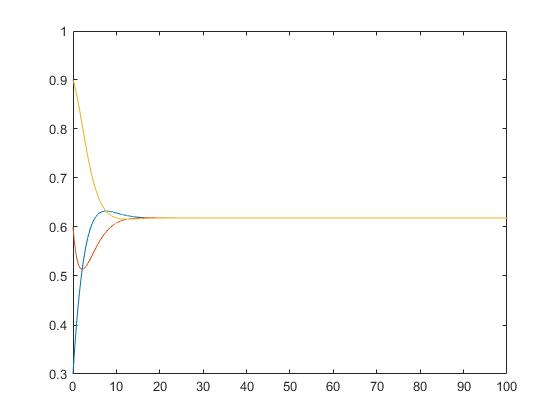
\includegraphics[scale=0.4]{1.jpg}
\caption{$x_0 = (0.3 \quad0.6\quad 0.9)$, $x^e = 0.6184178227652$}.
\end{figure}

The equilibrium in this case is from the space $U_e\ni x^e = 0.6184178227652$.




\newpage
If we change the initial conditions slightly the equilibrium point also changes. For example for the initial conditions
$x_0 = (0.35\quad 0.6\quad 0.9)$ the solutions converge to a different  equilibrium $x^e = 0.635643409191$
\begin{figure}[ht]
\label{fig_c2}
\centering
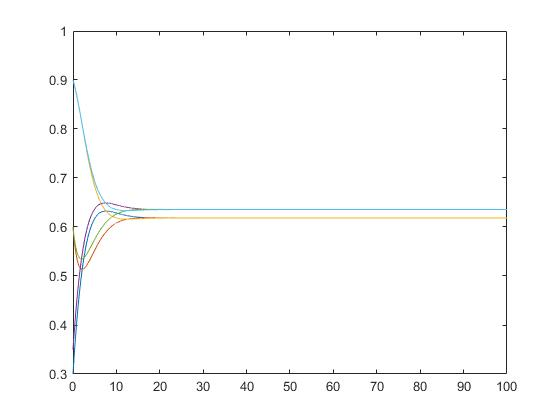
\includegraphics[scale= 0.4]{2.jpg}

\caption{$x_0 = (0.35 \quad0.6\quad 0.9)$, $x^e = 0.635643409191$}
\end{figure}

In (Fig. 2) the two solutions are plotted together for comparison.

\newpage

\subsection{Example 2}
To picture how the equilibrium space looks like, consider a two dimensional case  $N=2$, and let us plot the phase portrait of the system (\ref{s2}), for the time horizon $T = 10$, $x_{max} = 1$. and
$$
\mathbf{v} = 
\left(
\begin{matrix}
0 & 0.5  \\
0.5 & 0 \\
\end{matrix}
\right),
$$

$$
\mathbf{w} = 
\left(
\begin{matrix}
0.5 & 0 \\
0 & 0.5 \\
\end{matrix}
\right).
$$

\begin{figure}[ht]
\label{fig_c3}
\centering
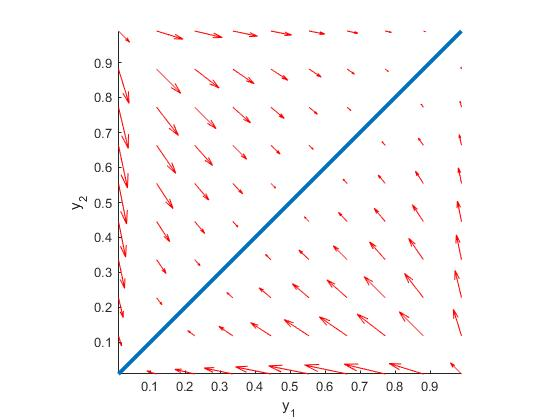
\includegraphics[scale= 0.4]{3.jpg}
\caption{Phase portrait}
\end{figure}

Here in  (Fig. 3) the thick bisectrice is the equilibrium space $U_e$, and and the red arrows show where the trajectories tend with time.
The trajectories along with the phase portrait are plotted on the following (Fig. 4)
\begin{figure}[ht]
\label{fig_c4}
\centering
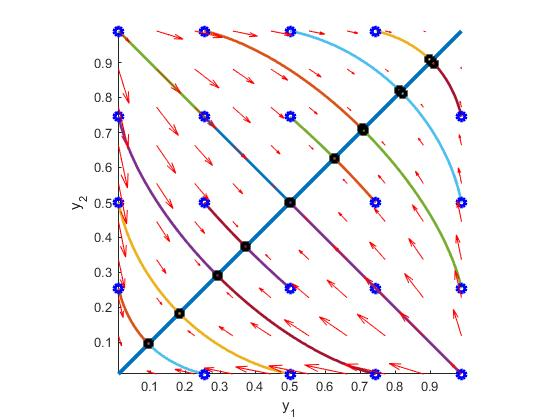
\includegraphics[scale= 0.4]{4.jpg}
\caption{Phase portrait along with the trajectories}
\end{figure}
where the blue circles denote the beginning of the trajectories and the dark squares denote the end of the trajectories.

The trajectory portrait in the $3-dim$ case in the first example is pictured on the following figure

\begin{figure}[ht]
\label{fig_c4}
\centering
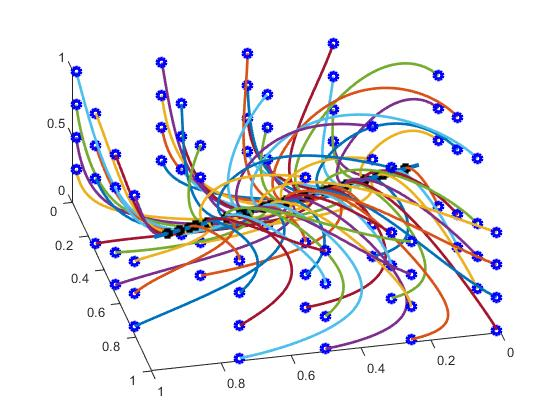
\includegraphics[scale= 0.4]{5.jpg}
\caption{Trajectory portrait.}
\end{figure}

As can be seen all trajectories converge to the bisectrice of the first cuboid.
\subsection{Example 3}
The matrices $\mathbf{v}$ and $\mathbf{w}$ can also depend on time. Consider the case $N=3$, the time horizon $T = 300$, $x_{max} = 1$,



$$
\mathbf{v} = 
 \lambda(t)\left(
 \begin{array}{ccc}
0 & 0.5 & 0.5 \\
0.5 & 0 & 0.5 \\
0.5 & 0.5 & 0 \\
\end{array} 
\right) 
+ (1-\lambda(t))
\left( 
\begin{array}{ccc}
0.5 & 0.5 & 0 \\
0 & 0.5 & 0.5 \\
0.5 & 0 & 0.5 \\
\end{array} 
\right)
$$


Here $\mathbf{v}$ and $\mathbf{w}$ are stochastic, then $|\mathbf{\Delta}| = 0$. Therefore the problem has more than one equilibrium. 
Let us have a look at the graph of the solution with the initial conditions $x_0 = (0.3\quad 0.6\quad 0.9)$.




\end{document}
